\documentclass[fontsize=10pt,paper=a4,bibliography=totoc]{scrartcl}

%\usepackage[utf8]{inputenc}
%\usepackage[ngerman]{babel}
%\usepackage{amsmath}
%\usepackage{graphicx}
%\usepackage{units}

% packages  
\usepackage[utf8]{inputenc}
\usepackage[T1]{fontenc}
\usepackage{ae}
\usepackage{tabularx}
\usepackage{amsmath,amssymb}
\usepackage[pdftex]{graphicx}
\usepackage{subfigure}
\usepackage{url}
\usepackage[T1]{fontenc}
\usepackage{ifthen}
\usepackage{hyperref}
\usepackage[absolute,overlay]{textpos}
\usepackage{tikz}
\usepackage[ngerman]{babel}
\usepackage{units}
\usepackage{bibgerm}
\usepackage{epstopdf}

\graphicspath{{images/}}

\usepackage{url}
\title{Ausarbeitung\\Solarthermisches Kraftwerk}

\author{K. Franke, M. Dolgov, F. Achilles\\The Raymen}
\begin{document}
\maketitle

\section{Stand der Technik}

\subsection{Dish-Stirling Anlage}
Die Dish-Stirling Anlage besteht aus einem großen Parabolspiegel, der meistens aus mehreren kleinen Spiegeln zusammengesetzt wird. Im Brennpunkt befindet sich ein Stirling Motor, der aus der gebündelten Wärme Strom erzeugt. Damit die Strahlen sich immer im Brennpunkt treffen, wird der große Parabolspiegel mit der Sonne mitgedreht um immer senkrecht einfallende Strahlen zu erreichen. Für dieses Konzept ist somit immer eine zweiachsige Nachführung des Spiegels nötig, da nicht senkrecht einfallende Strahlen den Absorber des Stirling Motors verfehlen würden. Dieses Konzept funktioniert daher nur bei direkter Sonneneinstrahlung und nicht bei diffusem Licht. Vorteil dieses Kraftwerktyps ist die sehr kompakte Bauweise, so können diese Kraftwerke schon für Leistungen ab 5kW eingesetzt werden \cite{1}. Nachteil ist die Größe des großen Spiegels, der ja nach Sonnenstand wie ein Segel wirkt. Je nach Standort muss die Konstruktion für unterschiedlich starke Windlasten ausgelegt werden, die ein solches Projekt teuer machen.
 
\subsection{Parabolrinnenkraftwerke}
Bei Parabolrinnenkraftwerken wird das einfallende Sonnenlicht von gewölbten Spiegeln auf eine Linie fokussiert. Ein mit Öl gefülltes Absorberrohr verläuft entlang dieser Linie. Die durch das Öl transportierte Energie kann in einem Gas- und Dampfkraftwerk zur Stromerzeugung genutzt werden. Der Vorteil von Parabolrinnenkraftwerken gegenüber Dish-Stirling-Anlagen besteht darin, dass die Nachführung nur einachsig erfolgen muss und somit ein günstigeres System realisiert werden kann. Ein weiterer Vorteil ist, dass ein stationäres Kraftwerk verwendet werden kann, das an einer beliebigen Stelle platziert werden kann. 

\section{Vorstellung des Konzepts}
Es wurde zuerst untersucht wie sich schräg einfallende Strahlung auf den Fokuspunkt der Strahlen auswirkt. Für solche Versuche wurde ein Raytracing Programm in Matlab geschrieben, das beliebig viele Strahlen in einer beliebigen Richtung erzeugt, den Schnittpunkt mit einem Spiegel findet, die Reflexionsrichtung berechnet und alles grafisch darstellen kann. 
\begin{figure}[htb]
	\centering
	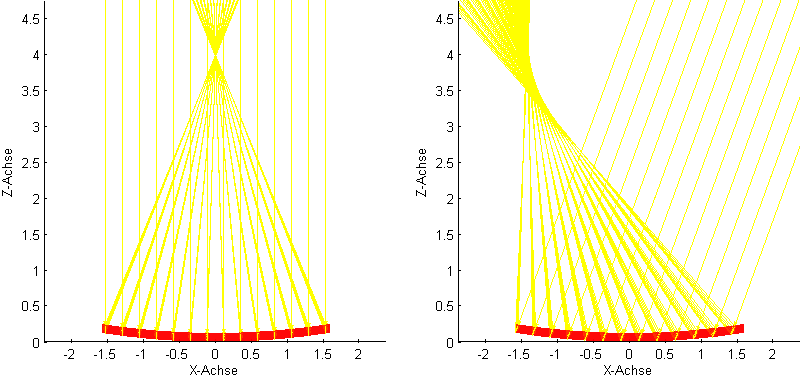
\includegraphics[width=\textwidth]{images/2d_gerade_schraeg20.png}
	\caption{Gerader Einfall auf Parabolspiegel}
	\label{pic:2dreflektion}
\end{figure}
Das Ergebnis ist in Abbildung~\ref{pic:2dreflektion} zu sehen. Während die Strahlen bei senkrechtem Lichteinfall genau im Fokuspunkt gebündelt werden, verschiebt sich dieser
bei schrägem Einfall nicht nur, die Strahlen werden nun auch nicht mehr so gut gebündelt, sondern fächern auf.

\subsection{Idee}
Die Hauptidee unseres Konzepts besteht darin die kompakte Bauweise einer Dish-Stirling-Anlage und stationäre Stromerzeugung eines Parabolrinnenkraftwerks mit möglichst geringen Kosten zu kombinieren. Die Anlage soll dabei aus einem großen, fest montierten Hauptspiegel sowie einem auf einer Schiene beweglichen kleineren Zweitspiegel bestehen, was in Abbildung~\ref{pic:system_rendered} veranschaulicht wird. Die Position des kleinen Spiegels kann also auf einer gegebenen Halbkugel frei eingestellt werden.
\begin{figure}[htb]
	\centering
	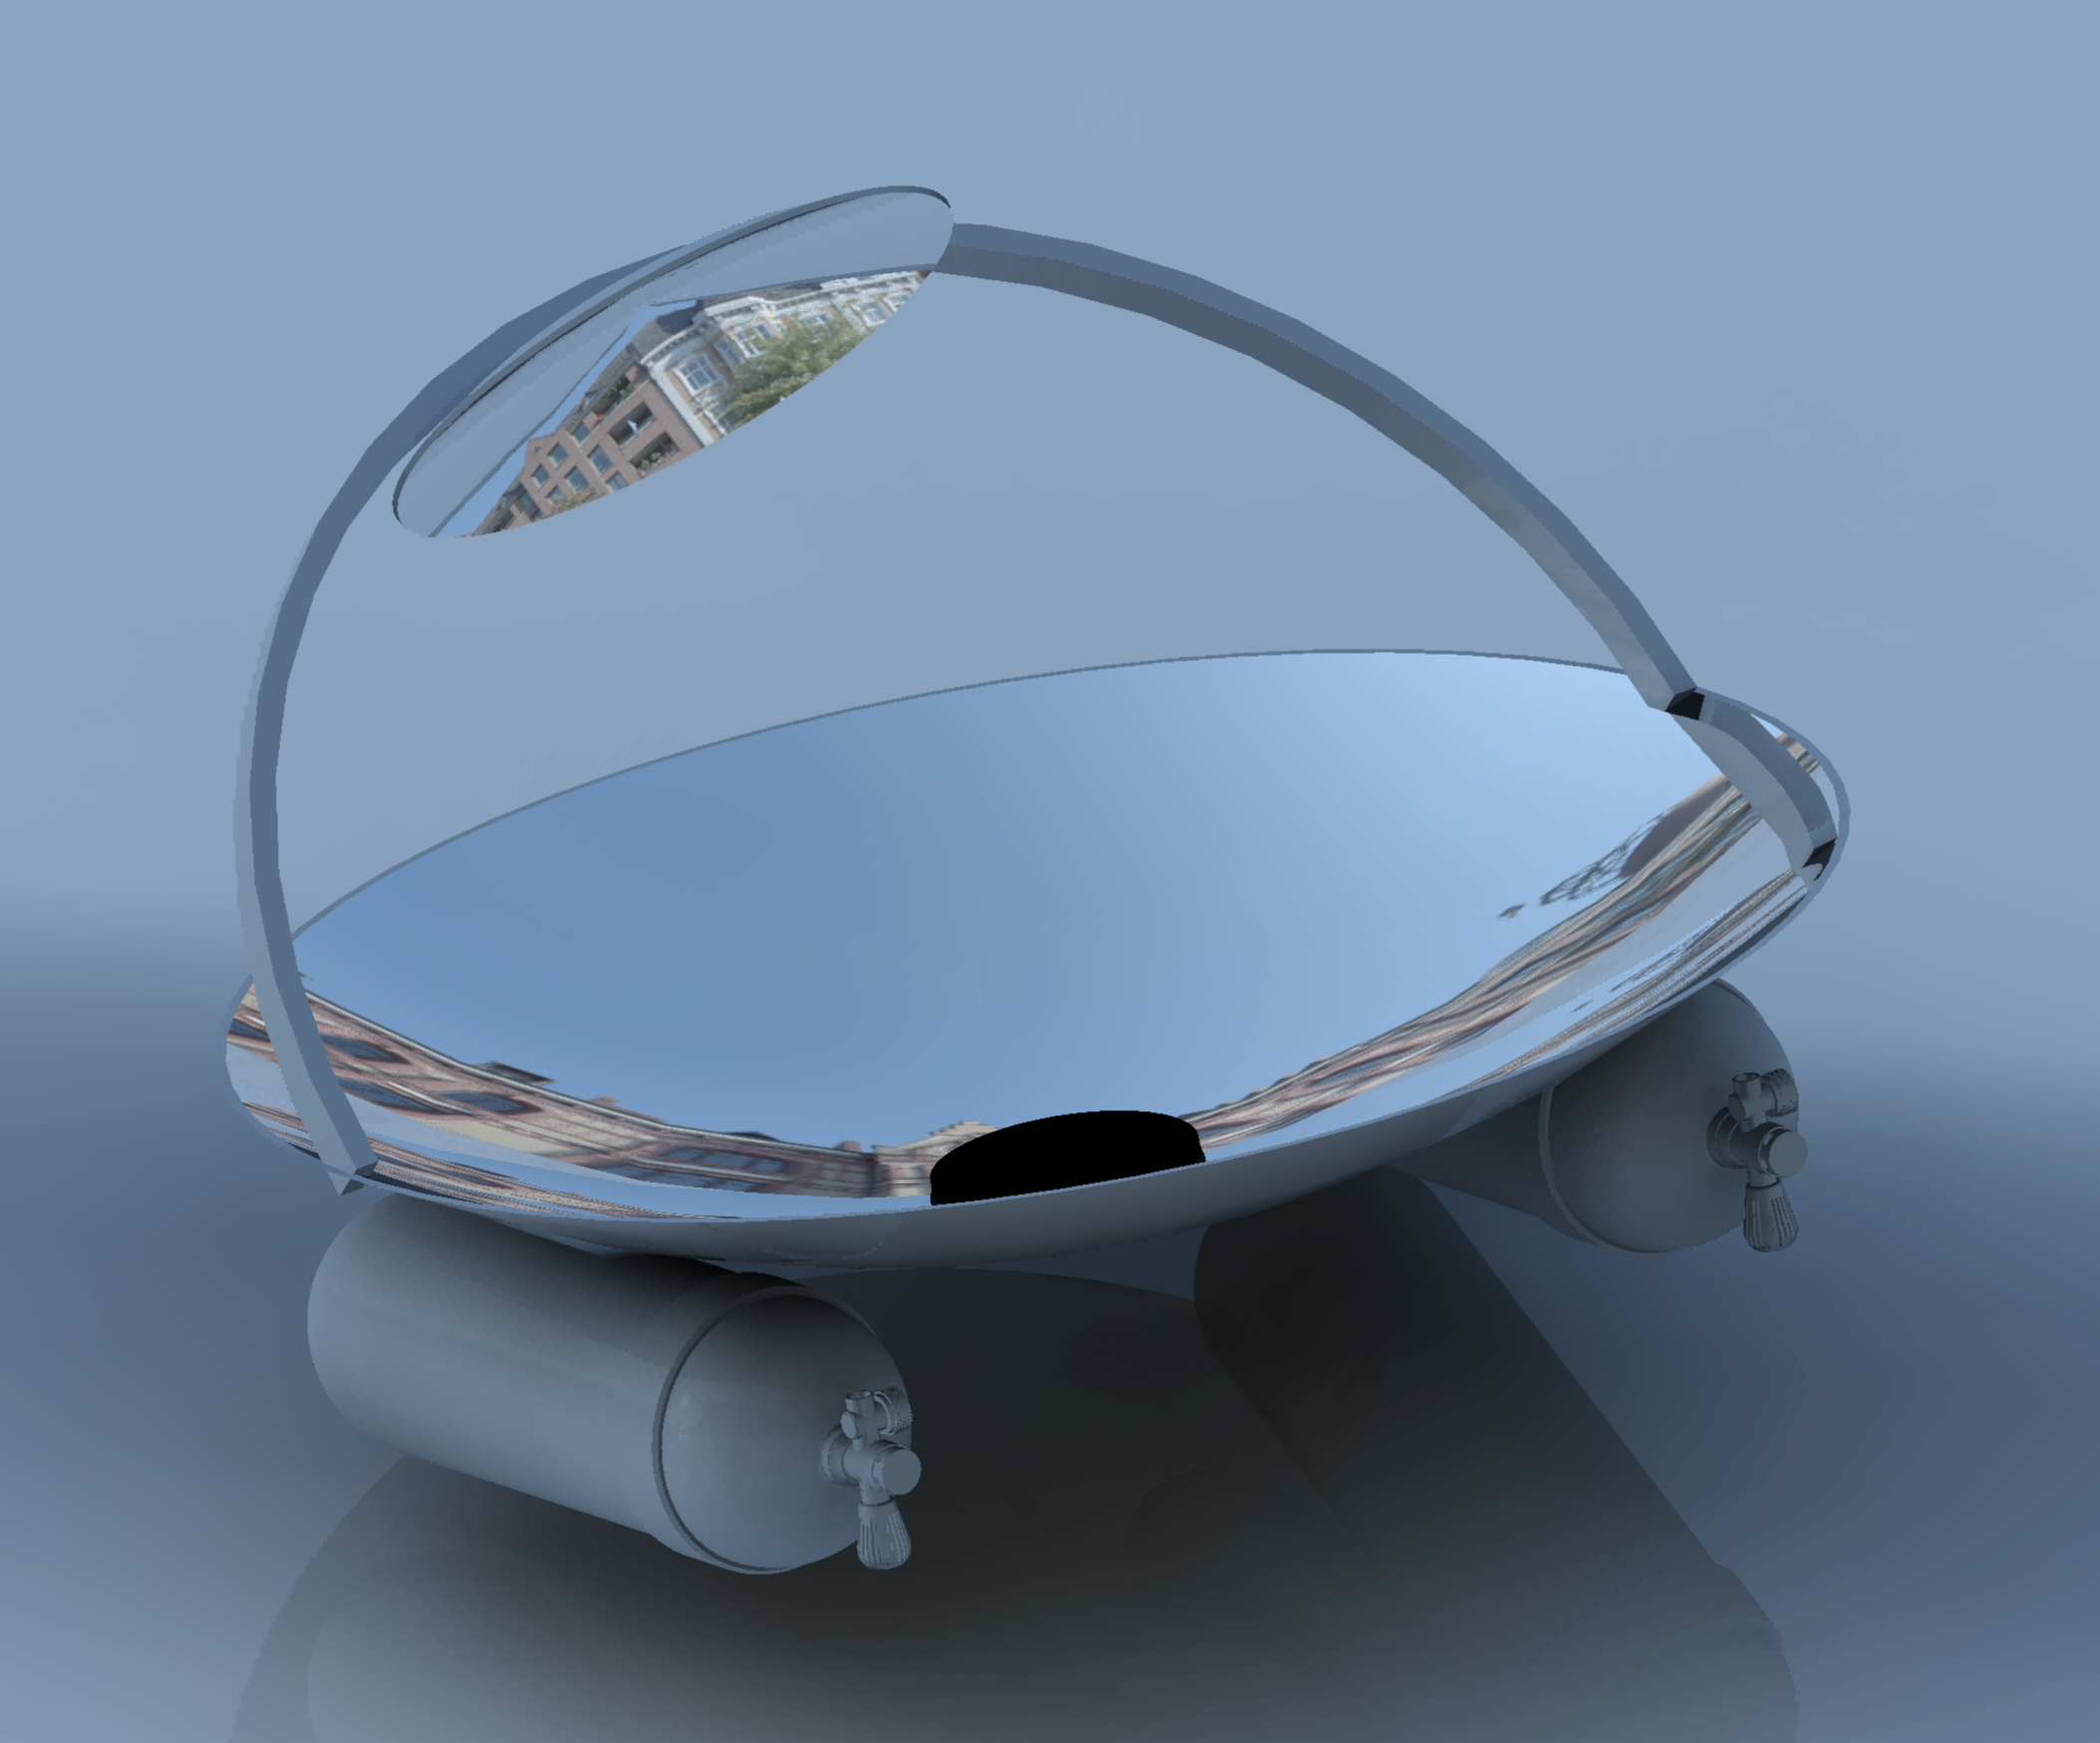
\includegraphics[width=\textwidth]{images/SMALL_MIRROR}
	\caption[Gesamtsystem]{Gesamtsystem mit großem und kleinen Spiegel, schwenkbarer Führungsschiene und Absorber.}
	\label{pic:system_rendered}
\end{figure}
Das einfallende Sonnenlicht wird zunächst vom Hauptspiegel reflektiert. Der Zweitspiegel folgt stets dem Fokuspunkt des Hauptspiegels, welcher seine Position abhängig von der Tages- und Jahreszeit verändert, und reflektiert das Licht anschließend zu einem in den Hauptspiegel integrierten Absorber.  Die im Absorber gesammelte Energie wird zur Stromerzeugung in einem stationären Kraftwerk verwendet.
Neben dem geschildertem Aufbau des Kraftwerks, wird ein Konzept zur Energiespeicherung in einem Luftdrucksystem vorgestellt, welches vor allem für Privathaushalte eine On-Demand-Stromerzeugung ermöglichen soll.

\subsection{Erhoffte Vorteile}
Es wird erhofft, dass der Konstruktionsaufwand durch einen stationären Hauptspiegel weitgehend gering ausfallen wird. Besonders soll hier hervorgehoben werden, dass der Hauptspiegel dadurch, dass er stationär ist viel einfacher die erforderlichen Windlasten aushält. Der Zweitspiegel kann sehr leicht gebaut werden und kann bei zu starkem Wind in den Schutz des Hauptspiegels gefahren werden. Die Motoren zur Nachführung des kleinen Spiegels können sehr klein ausgelegt werden. Unter dem Absorber soll direkt die Umwandlung in elektrischen Strom geschehen, was die Transportwege verkürzt und die Komplexität verringert. 

\section{Beschreibung des Programms}
Zur Berechnung der Geometrie des beschriebenen Zweispiegelsystems wurde ein Mat"-lab-Programm geschrieben. Dieses berechnet die optimalen Formen der Spiegel durch Lösen eines Maximierungsproblems, welches darin besteht, eine möglichst große Strahlendichte pro Absorberfläche zu erhalten. Nachfolgend wird die Vorgehensweise des Unterprogramms beschrieben, das bei jeder Optimierungsiteration aufgerufen wird. Die einzelnen Blöcke werden anschließend erklärt.
\subsection{Ablaufdiagramm (Top-Level)}
\begin{figure}[htb]
	\centering
	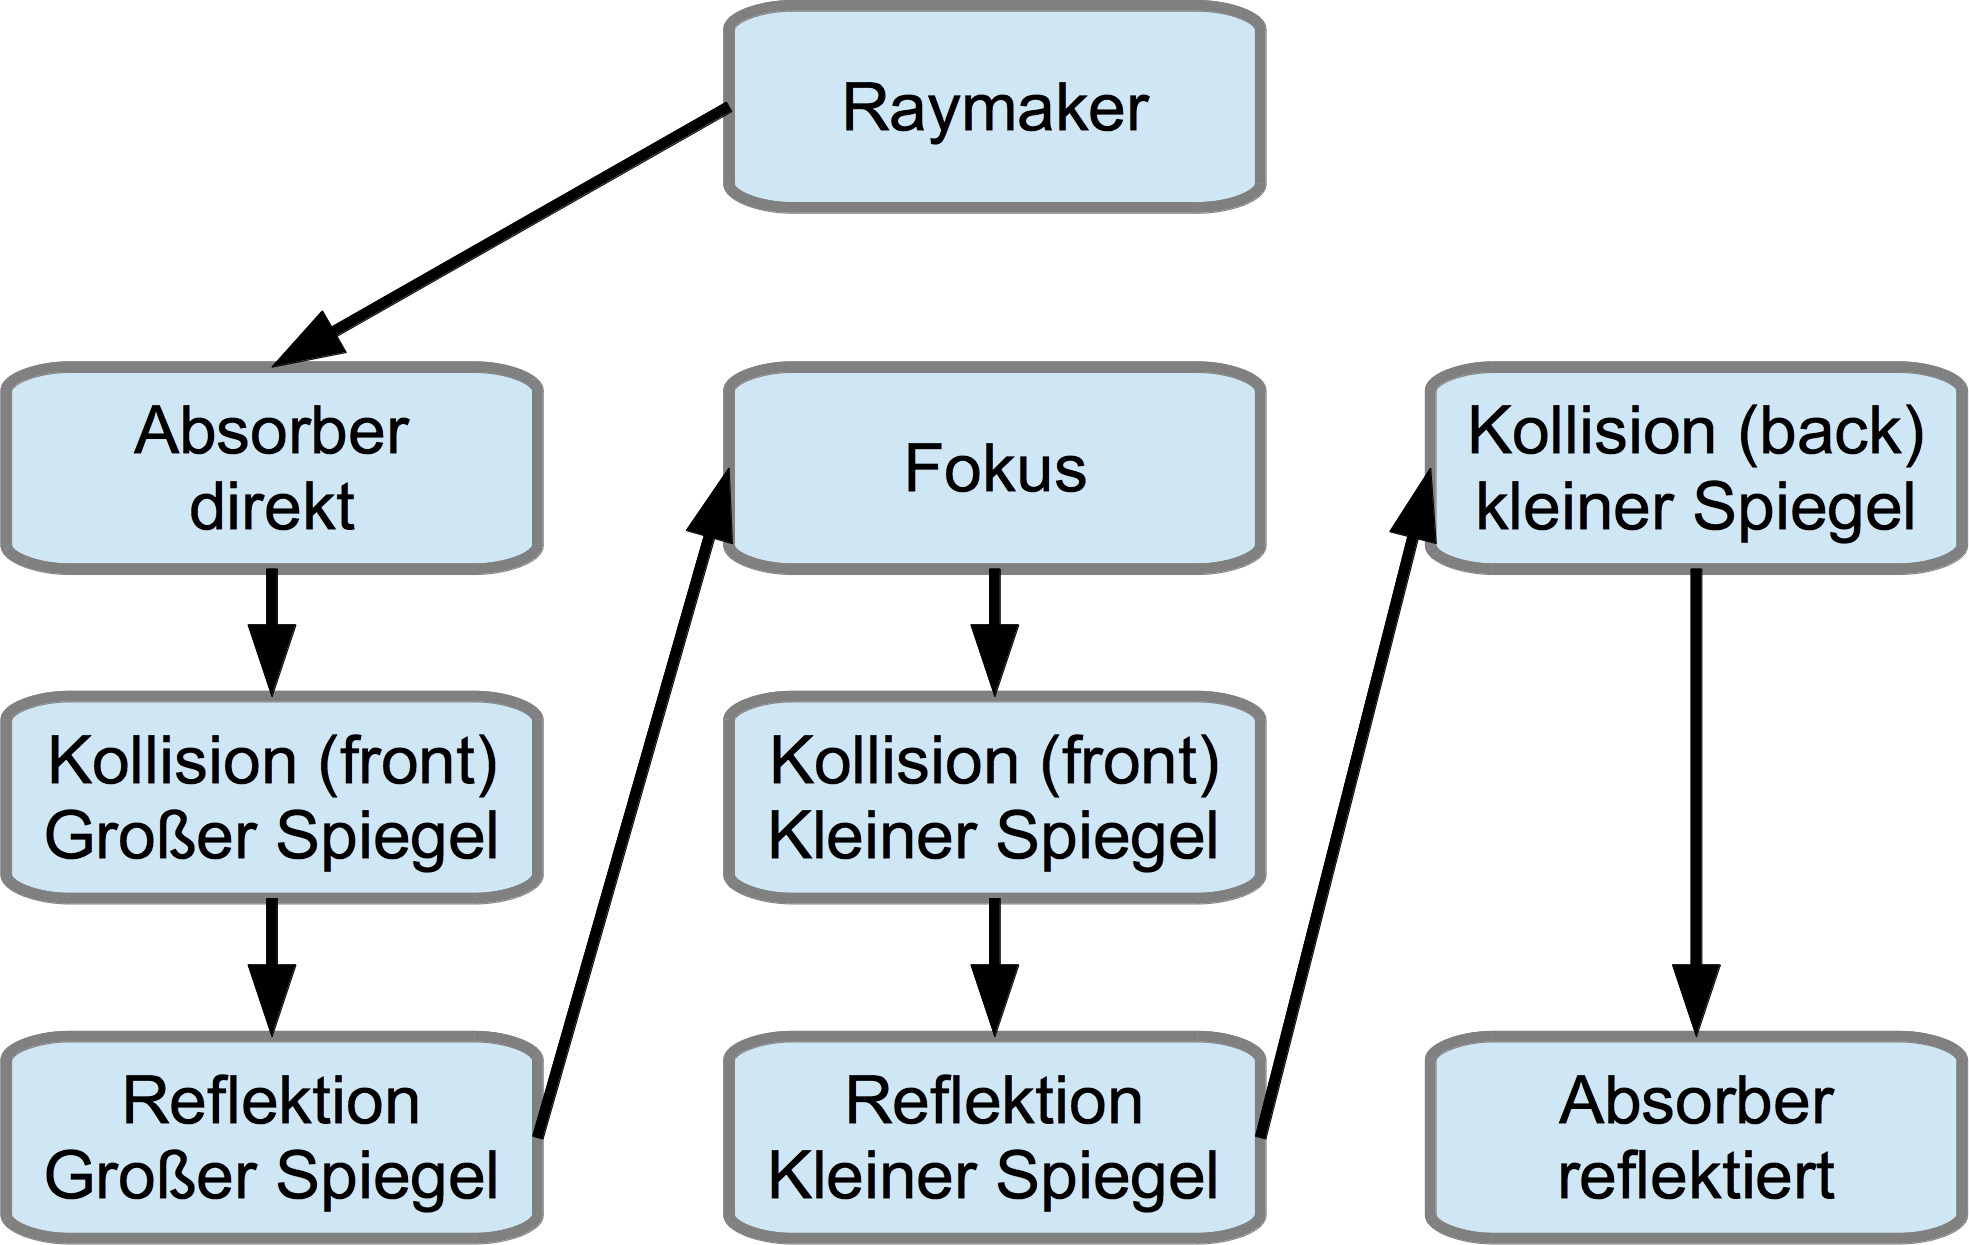
\includegraphics[width=0.7\textwidth]{images/Diagramm.png}
	\caption{Ablaufdiagramm für Raytracer}
	\label{pic:Raytracer}
\end{figure}
\subsection*{Kollisionsdetektion}
Eine Kollision von Strahlen und Spiegelfläche muss zu vier Zeitpunkten des Programms überprüft werden:
\begin{enumerate}
\item Kollision am Hauptspiegel,
\item Kollision am kleinen Spiegel (blockierende Rückseite),
\item Kollision am kleinen Spiegel (spiegelnde Vorderseite),
\item Absorption in der Absorberfläche.
\end{enumerate}
Der Collision Tracker folgt zunächst der Richtung jedes Strahls in einer festgelegten Schrittweite. Sobald eine Höhe $Z_{unter}$ erreicht wird, die kleiner als die Spiegelhöhe $Z_{Spiegel}$ an diesen Koordinaten ist, hat der Strahl den Spiegel durchstoßen.
Darauf beginnt die zweite Art der Suche, bei der der Suchraum mit jedem Schritt halbiert wird. Diese Dychotome Suche vergleicht, ob die Mitte zwischen zwei Randpunkten über oder unter dem Spiegel liegt. Ein Randpunkt ist dabei der soeben erreichte $Z_{unter}$, der zweite ist der Punkt $Z_{ueber}$, der vor dem Durchstoßen erreicht wurde. Zwischen diesen beiden Grenzen muss zwangsweise der Kollisionspunkt liegen, der mit beliebiger Genauigkeit gefunden wird. 

\subsubsection*{Reflexion}
Die Reflexion kann entweder am Hauptspiegel oder am kleinen Spiegel erfolgen. Zur Berechnung der reflektierten Richtung wird die Normale des Spiegels am Kollisionspunkt bestimmt und dann mit Hilfe des Kreuzprodukts berechnet.

\subsubsection*{Raymaker}
In dieser Funktion werden Strahlen nach dem tatsächlichen Sonnenverlauf generiert. Diese entstehen in einer festen Höhe über dem Hauptspiegel und können je nach gewünschter Strahlendichte und Richtung erzeugt werden.

\subsubsection*{Fokusbestimmung}
Die Fokusbestimmung bestimmt die Position des kleinen Spiegels. Sie berechnet zuerst den Mittelwert aller Kollisionspunkte auf dem Hauptspiegel und anschließend den Mittelwert ihrer Richtungen. Der sich ergebende Vektor aus gemitteltem Kollisionspunkt und gemittelter Richtung ist der gewünschte Fokus. Dieser wird skalar so erweitert, dass er die Halbkugel schneidet, die vom kleinen Spiegel angefahren wird.

\section{Stromerzeugung}
Im folgenden wird ein Konzept zur Stromerzeugung und Energiespeicherung vorgestellt.
\subsection{Energieumwandlung über Pressluft}
Ähnlich wie bei einem Solar-Stirling ist die Idee Luft als Arbeitsmedium zu verwenden.
Die Luft befindet sich dabei in einem großen Pressluftbehälter der als Druckluftspeicher dient. Um gängige Standards verwenden zu können, die keine regelmäßigen TÜV-Inspektion benötigen, und um vor allem günstig und einfach zu sein, wird in dem im Heimwerker-Bereich üblichen Druckbereich von ca. 12 Bar gearbeitet.
Die Luft soll dann über einen Wärmetauscher mit mehreren in Reihe geschaltete Wärmespeichern geleitet werden, um so bei einem geringen Temperaturgradient die Luft zu erhitzen und so den Druck weiter zu erhöhen.

\subsection{Wärmespeicher}
Als billigster und dennoch sehr speicherfähiger Wärmespeicher bietet sich in erster Linie Wasser an (4,182 kJ/(K*kg) ). Da wir jedoch um höhere Wirkungsgrade zu erreichen mit möglichst hohen Temperaturdifferenzen arbeiten müssen, können wir nicht alleine mit Wasser als Wärmespeicher arbeiten, da dieses ab $100^\circ$C verkocht.
Ein Baustoff der recht einfach zu handhaben sein sollte und verhältnismäßig billig ist, ist Beton. Er kann vor Ort beim Errichten der Solaranlage selber angemischt werden oder vorab in einzelne Module, in der Größe von Steinfließen vorgefertigt werden.
Den Beton kann man dabei aus Zement und anderen günstigen Baustoffen wie Sand und Steinen zusammenmischen um Geld zu sparen. Diese Baustoffe haben alle eine ähnliche spezifische Wärmekapazität um die 0,88kJ/(K*kg) bei eine Dichte von $2,4\frac{t}{m^3}$ \cite{waerme}.
Jedoch muss man auch bei dem Beton Acht geben. Wenn man ihn auf hohe Temperaturen erhitzt (600K!) kann das Wasser aus dem Beton freigesetzt werden. Es gibt hierzu Forschung für spezielle Beton als Wärmespeicher  \cite{speicher}  \cite{beton};
“Der Beton kann sich dabei theoretisch auf bis zu $1000^\circ$C erhitzen, praktisch werden bisher aber nur ca. $400^\circ$C erreicht.”
Das sollte im Rahmen liegen in dem Modell wurden zum Test Temperaturen bis 600K eingegeben.
Das Gewicht des Wassers und des Beton nutzt gleichzeitig als Ballast, so dass die Konstruktion Wind standhalten sollte.
Als Wärmetauscher bieten sich Kupferrohre an. Sie haben eine hohe Wärmeleitfähigkeit ca. 300 W/m*K

\subsection{Prozess}
Die Luft die zuvor in den Presslufttanks Raumtemperatur hatte wird so durch den Wärmetauscher geleitet, dass sie zuerst einen Wärmetauscherbereich mit thermischen Kontakt zur Umgebungsluft, dann durch eine Reihe immer wärmer werdenden Wasserwärmespeichern und dann zum Betonwärmespeicher geleitet wird. Zuletzt durchläuft die Luft einen Bereich indem sie in thermischen Kontakt mit dem Absorber kommt.
Wir nehmen bei einer Reflektorfläche von $4m^2$ bei direkter Sonneneinstrahlung etwa 3000W an.
Funktionsprinzip

\section{Ergebnisse}
Bis zu diesem Zeitpunkt (\today) haben wir einige Szenarien der Optimierung durchgerechnet. Die grundlegende korrekte Funktion des Raytracers soll in Abbildung~\ref{pic:netteReflektion} verdeutlicht werden. Nur Sonnenstrahlen, die den blau dargestellten Absorber treffen, sind abgebildet. Der große und kleine Spiegel haben jeweils Parabolform , dabei wird die Grundfläche des großen Spiegels von den vorgegebenen \unit[10]{m$^2$} begrenzt.
\begin{figure}[htb]
	\centering
	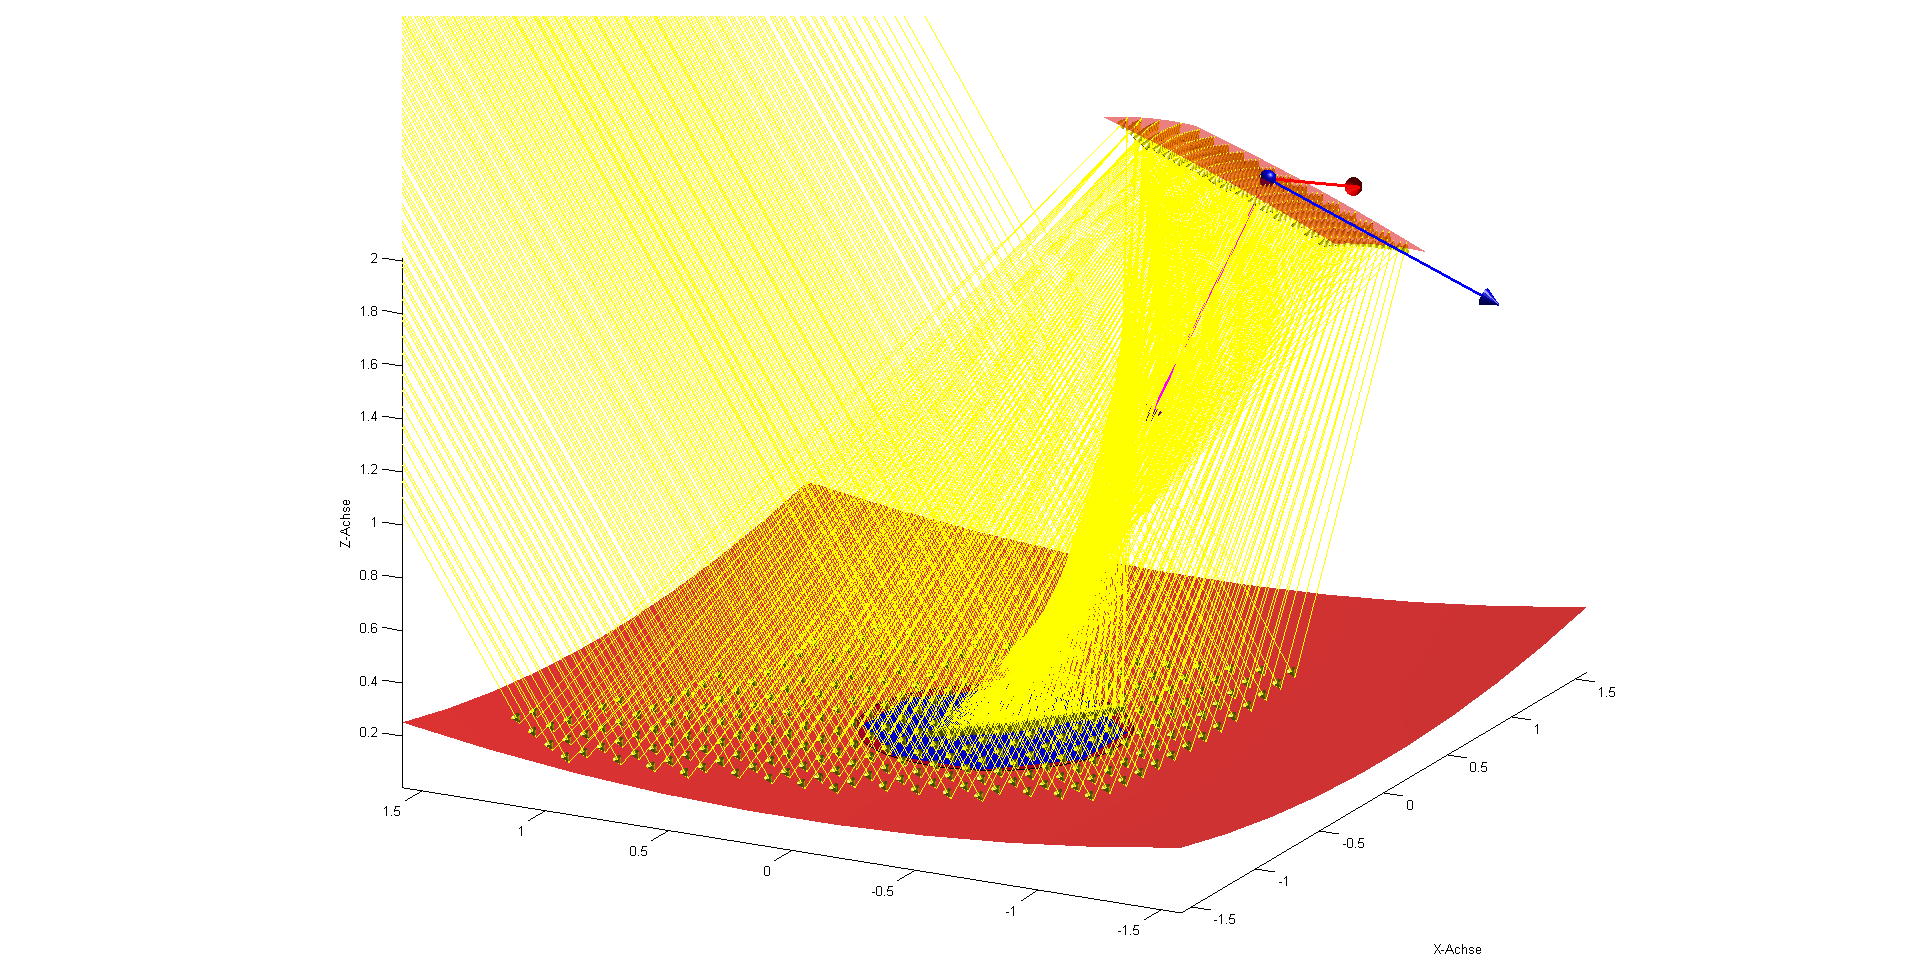
\includegraphics[width=\textwidth]{images/netteReflektion}
	\caption[Bündelung schräg]{Schräger Einfall auf Parabolspiegel, Reflektion und Bündelung durch zweiten kleineren Spiegel.}
	\label{pic:netteReflektion}
\end{figure}
Zu erkennen ist die korrekte Verschiebung des kleinen Spiegels an den Ort des verschobenen Fokuspunktes (vgl. Abb.~\ref{pic:2dreflektion}), sowie dessen Ausrichtung auf den Absorber.
Ungefähr \unit[40]{\%} der zur Verfügung stehenden großen Spiegelfläche werden von Strahlen getroffen, die den Absorber erreichen. Dies entspräche also einem Wirkungsgrad $\eta_{Sonne}$ von \unit[40]{\%}. Für eine Abschätzung des Gesamtwirkungsgrades $\eta_{gesamt}$ muss noch der Wirkungsgrad des nachgeschalteten Generators multipliziert werden.

\bibliographystyle{ieeetran}
\bibliography{bib}

\end{document}